\begin{figure*}[ht]
\centering
\begin{subfigure}{.33\textwidth}
  \centering
  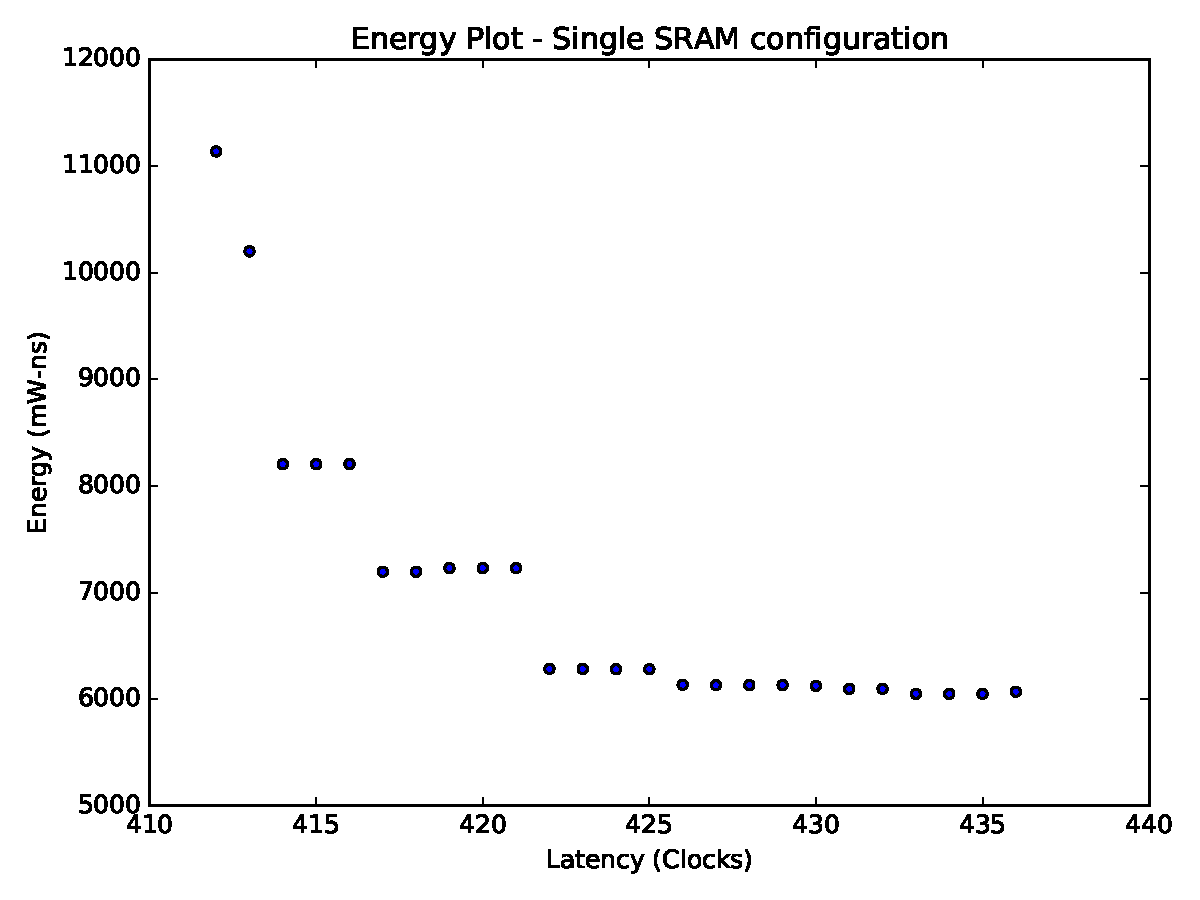
\includegraphics[width=\textwidth]{graphs/energy_plot_single_sram.pdf}
  \caption{5x5 MM}
  \label{fig:single_sram}
\end{subfigure}%
\begin{subfigure}{.33\textwidth}
  \centering
  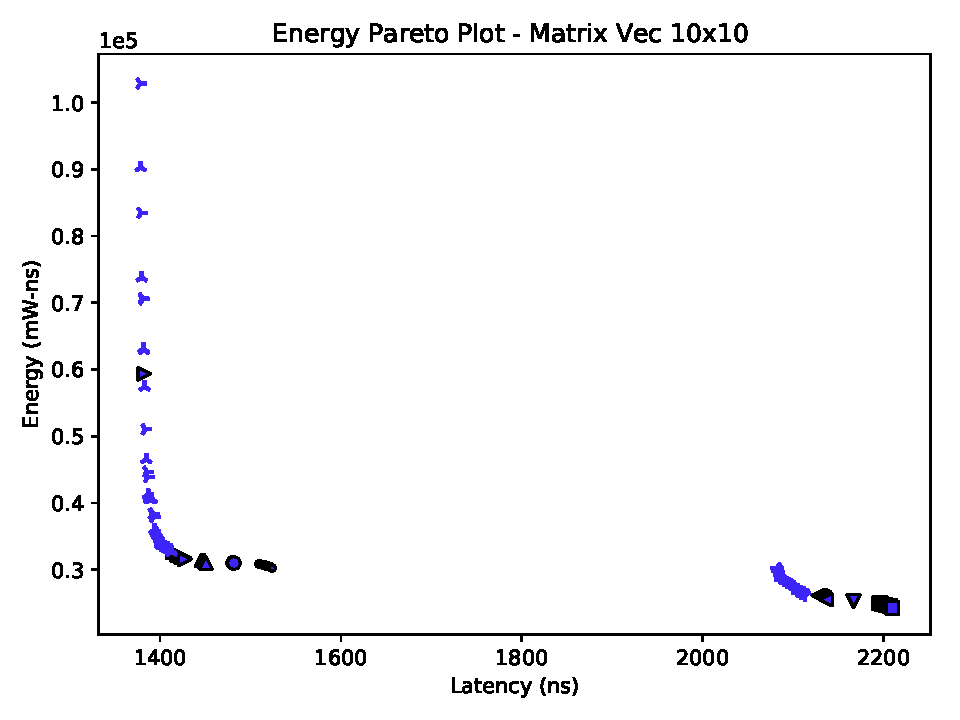
\includegraphics[width=\textwidth]{graphs/EnergyParetoMatrixVec10.pdf}
  \caption{MV 10x10}
  \label{fig:sram_vs_mram_pareto_vec}
\end{subfigure}
\begin{subfigure}{.33\textwidth}
  \centering
  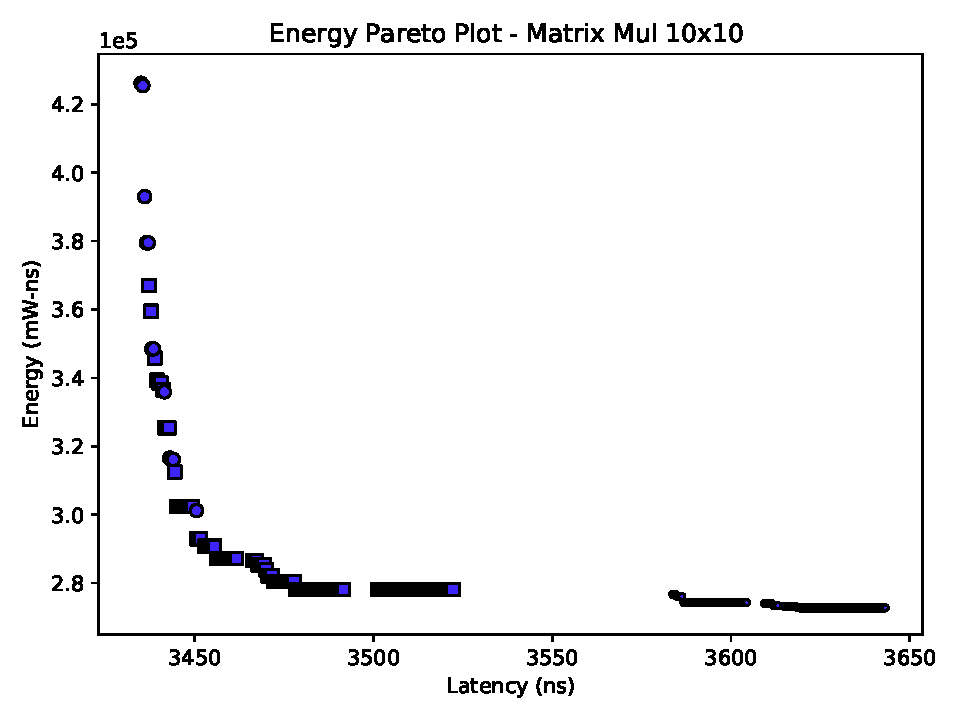
\includegraphics[width=\textwidth]{graphs/EnergyParetoMatrixMul10.pdf}
  \caption{MM 10x10}
  \label{fig:sram_vs_mram_pareto_mul}
\end{subfigure}
    \caption{\small Each point represents one \frameworkname~custom-processor. Different shapes (in \ref{fig:sram_vs_mram_pareto_vec} and~\ref{fig:sram_vs_mram_pareto_mul}) identify different input configurations. \ref{fig:single_sram} shows the architecture's Energy over Latency in clock cycles generated from a single configuration of a matrix vector multiplication of size 5x5. Note that (a) presents all designs, while (b) and (c) only include the Pareto-optimal designs.}
\label{fig:case_studies_1}
\end{figure*}
\section{Case Studies}
\label{sec:case_studies}
In this section we demonstrate the capabilities of \frameworkname~using three case studies. To do so, we analyze the architectures generated by \frameworkname~and we analyze the energy consumption and latency of each design.
We selected two representative applications: matrix-vector (MV) and matrix-matrix (MM) multiplication. The matrix sizes are 5x5, 10x10, and 15x15. We used the TSMC 28nm target technology library for generating the database containing the area usage and energy consumption of the different building blocks, as required by our framework.
We generated multiple input \textit{Configuration Parameters} - Section~\ref{ssec:conf_param} - to let \frameworkname~select the correct building blocks data from the database, and compute the latency, area usage, and energy consumption of the architectures. Each generated architecture has a known latency imposed in each iteration of the DSE(Section~\ref{ssec:dse}), which we use to compute its static energy consumption. Moreover, after applying the Modified Interval Partitioning algorithm (see Section~\ref{ssec:modified_interval_partitioning}), the instructions performed by each FU are known and this information is used to compute the dynamic energy consumption of an architecture.

In the first case study - Section~\ref{ssec:exp_single} - we illustrate how DSE works for 5x5 MV and a single configuration. The second case study compares the use of MRAM - modeled according to~\cite{8310393} - and SRAM for L2M (both in 28nm) for the two applications. The last case study compares \frameworkname~architectures for the different MV sizes.

\vspace{-1mm}
\subsection{Single configuration DSE}
\label{ssec:exp_single}
\vspace{-1mm}
The goal of this case-study is to illustrate the ability of \frameworkname~to generate, given a single configuration, architectures with varying energy consumption. The configuration uses SRAM in both levels. L2M is clocked at 350MHz, while L1M and the custom processor are clocked at 1GHz. Figure 7a shows the energy consumption of 30 different \frameworkname~designs, with 30 latencies. We make two observations: (1) the designs' latencies and power consumption range between the min and max latency, as given by the \textbf{MostPar} and \textbf{MostSeq} architectures, and (2) as expected, faster designs exhibit higher energy consumption, due to their larger numbers of FUs.

%The \textbf{MostPar} - starting point of our DSE - is the fastest architecture completing the computation in 412 clock cycles of the custom processor and it consumes $11.1^3$ mW-ns. The \textbf{MostSeq} - ending point of the DSE - is the slowest, completing in 436 clock cycles and consuming $6^3$ mW-ns. Between these two extreme design points, the DSE generates intermediate architectures with various energy-latency tradeoffs.

\vspace{-1mm}
\subsection{MRAM vs SRAM Level 2 Memory}
\label{ssec:case_study2}
\vspace{-1mm}

In this case study we compare the power efficiency of two alternative technologies to implement L2: MRAM and SRAM.
The comparison is performed using both applications - MV and MM - with 10X10 matrices (see Fig~\ref{fig:sram_vs_mram_pareto_vec} and~\ref{fig:sram_vs_mram_pareto_vec}, respectively). In both graphs, each point is relative to a hardware architecture generated by \frameworkname; moreover shapes identify different input configurations. Specifically, we compare a total of 18 configurations: 2 L2M technologies, MRAM and SRAM, clocked at 350MHz, and 9 different clock frequencies (400MHz - 1GHz, in steps of 200) for the processor and L1M ensemble.

In both figures we can identify two clusters: HE-LL (high-energy, low-latency) and LE-HL (low-energy, high-latency). Each cluster belongs to one memory technology: HE-LL contains of all SRAM designs, while LE-HL containts all MRAM designs.
For the MV application (Fig~\ref{fig:sram_vs_mram_pareto_vec}) the fastest architecture - using SRAM memory - has a latency of 1375ns and consumes over $1^5$mW-ns. The most energy efficient SRAM architecture has instead a latency of 1525ns and consumes under $0.3^5$mW-ns, thus being 3x more energy efficient than the fastest with a 10\% increase in latency. The most energy efficient architecture using MRAM technology has instead a latency of 2210ns and consumes $0,24^5$mw-ns, hence having 45\% higher latency than the best SRAM counterpart, with 25\% decrease in power consumption. The matrix multiplication, Figure~\ref{fig:sram_vs_mram_pareto_mul}, performs 10 times more operation than the matrix vector multiplication, hence there is a clear overall increase in latency - about 30\% - and energy consumption - about 4 times -  in comparison to the previous application. In this case the architecture using SRAM consuming the least amount of energy is has 2\% higher latency compared to the fastest one, but consumes 50\% less energy. However, the introduction of MRAM technology in the L2M is not as beneficial as it was for the matrix vector application. The MRAM architecture consuming the least amount of energy has a 3\% slowdown compared to the most energy efficient SRAM, while attaining only a 2.2\% improvement in energy consumption.

\begin{table*}[!ht]
  \resizebox{\textwidth}{!}{%
\begin{tabular}{llllll}
Framework & Type (see \ref{sec:bg})    & Application Optimized & Memory Co-Design & Architectural DSE & High Level Language \\
\frameworkname         & Distributed Control       & Yes                   & Yes              & Yes               & Yes, C              \\
\cite{parashar2014efficient}               & Distributed Control       & No                    & No               & No                & No                  \\
\cite{prabhakar2017plasticine}               & Centralized Control       & No                    & No               & No                & Yes, DHDL           \\
\cite{streamproc2019}               & Distributed Control       & No                    & No               & No                & No           \\
\cite{budiu2004spatial}               & Design-Time Programmable & Yes                   & No               & No                & Yes, C
\end{tabular}
}
\caption{Comparison with related work.}
\label{tab:rw}
\end{table*}

\subsection{Different Matrix Dimensions}
In this case study we compare three different matrix sizes for MV - 5x5, 10x10 and 15x15, using the same configurations used in~\ref{ssec:case_study2}, to evaluate how the energy consumption of an L2M MRAM scale with respect to an L2M SRAM. Figure~\ref{fig:sram_vs_mram_pareto_vec_sizes} shows the Pareto-optimal architectures generated from each input application. The increase in the matrix size is reflected by an increase in latencyi: all MV-5x5 custom-processors have latencies below 1000ns, MV-10x10 processors latencies range between 1250ns and 2500ns, and the MV-15x15 processors have latencies beyond 2500ns.
However, the increased number of operations results instead in wider tradeoffs possibilities. Thus, the normalized latency gap between the most energy efficient SRAM and MRAM, decreases with the matrix size, from 82\% for the 5x5, to 42\% for the 10x10 and even 32\% for the 15x15. The reduction in energy consumption between the same pair of results is instead 20\% for the 5x5 and 10x10, while for the 15x15 drops to 16\%. Therefore, as the size of the matrix grows, the benefits in energy consumption when using MRAM technology in the L2M reduce. This is a behaviour caused by the increased number of write operations that have high energy impact when the MRAM technology is used.



\begin{figure}[!h]
\centering
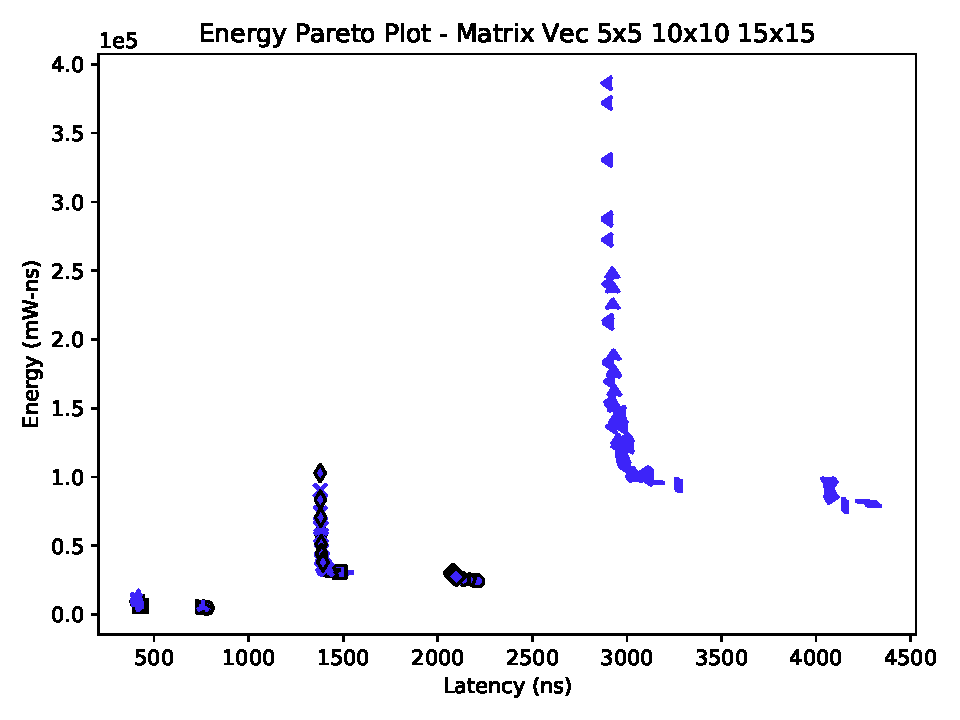
\includegraphics[width=0.33\textwidth]{graphs/EnergyParetoPlotMultipleSizeMAtrixVec.pdf}
    \caption{\small Energy Pareto optimal architectures generated by \frameworkname ~for different sizes of Matrix Vector multiplication 5x5 - with latencies ranging from 0 to 1000,10x10 - having latencies between 1000ns and 2500ns , and 15x15- with latencies above 2500ns. Each point corresponds to an architecture generated by the framework.}
\label{fig:sram_vs_mram_pareto_vec_sizes}
\end{figure}
